Thinking...
We need to translate Japanese sentence(s) to English, preserving TeX code unchanged. The Japanese text: "以下のの日本語文を英訳してください。ただしTeXのコードが挿入されているのでその部分はそのまま出力してください："

Then the TeX block includes caption in Japanese: "累積世代、論文グループごとの研究テーマの出現に関するエントロピー". Need to translate that caption to English, while leaving rest unchanged.

Thus output should be same TeX block but with caption translated. Also maybe translate any other Japanese text outside? The instruction is to translate Japanese sentences, but only caption is Japanese inside TeX. The surrounding instruction can be omitted; just output the translated block.

So we output:

\begin{figure*}[h]
\begin{center}
{\small
\begin{tabular}{ccc}
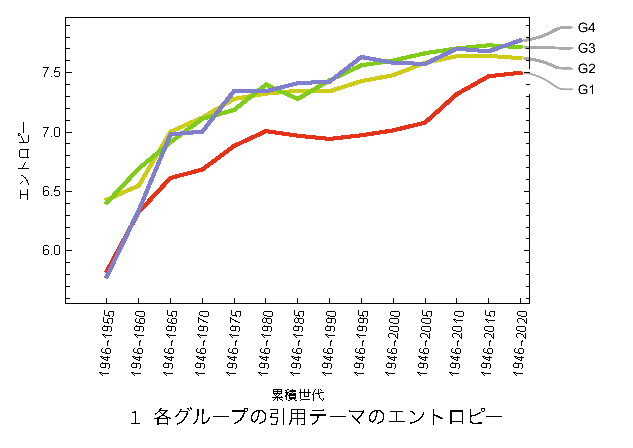
\includegraphics[width=51mm]{entropymesh-1.eps} &
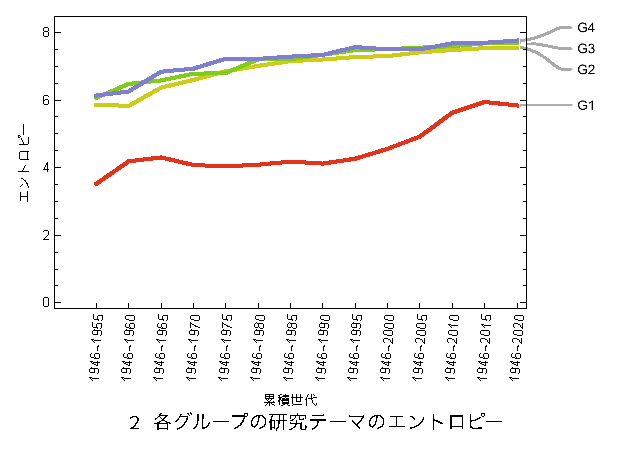
\includegraphics[width=51mm]{entropymesh-2.eps} &
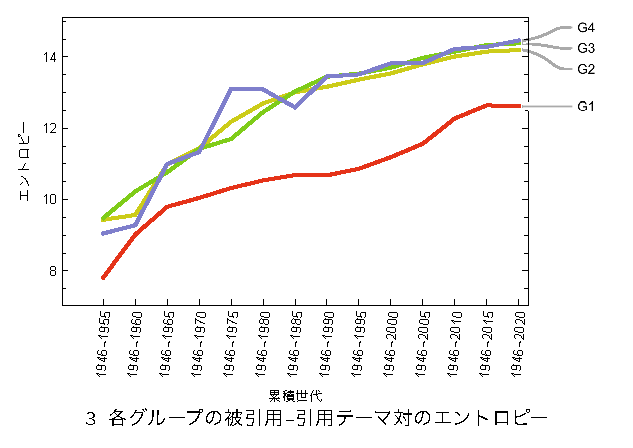
\includegraphics[width=51mm]{entropymesh-3.eps} \\
\end{tabular}
}
\caption{Entropy of the occurrence of research topics by cumulative generation and by paper group}
\label{fig:arr2}
\end{center}
\end{figure*}

Make sure translation is accurate: "累積世代、論文グループごとの研究テーマの出現に関するエントロピー". Could be "Entropy concerning the occurrence of research topics across cumulative generations and per paper group". A smoother: "Entropy of research topic occurrences across cumulative generations and for each paper group". We'll produce a natural translation.

Thus final.
...done thinking.

\begin{figure*}[h]
\begin{center}
{\small
\begin{tabular}{ccc}
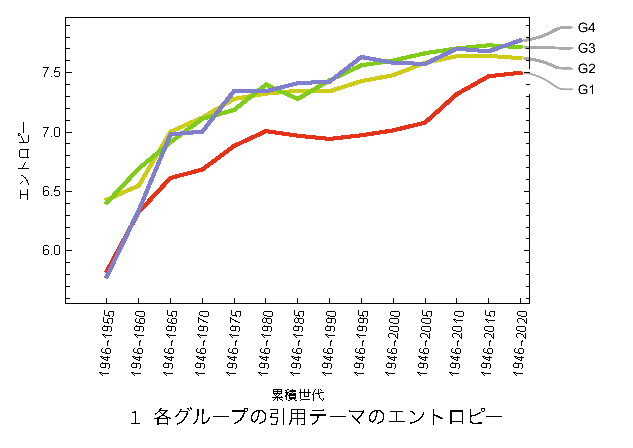
\includegraphics[width=51mm]{entropymesh-1.eps} &
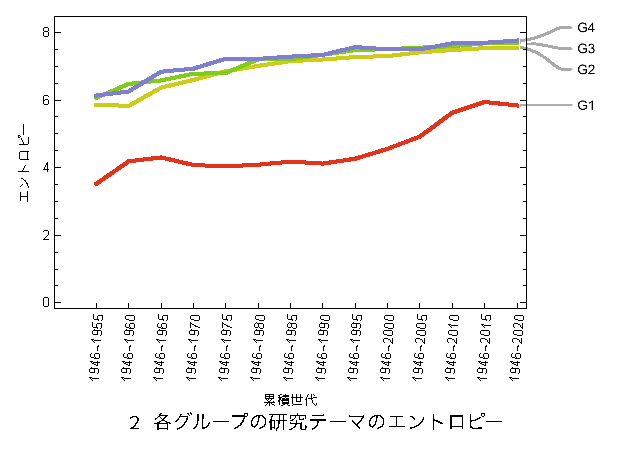
\includegraphics[width=51mm]{entropymesh-2.eps} &
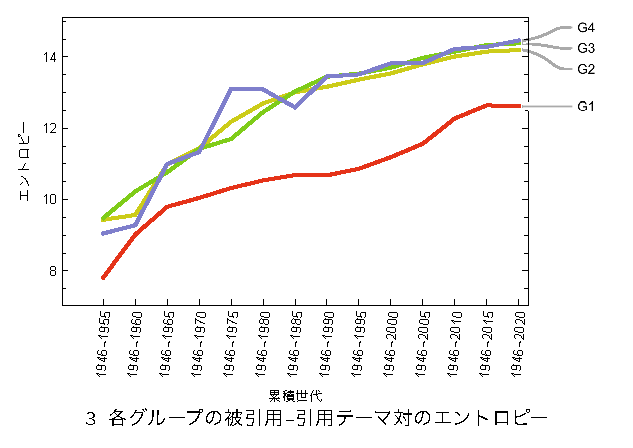
\includegraphics[width=51mm]{entropymesh-3.eps} \\
\end{tabular}
}
\caption{Entropy of research‑topic occurrences across cumulative generations and for each paper group}
\label{fig:arr2}
\end{center}
\end{figure*}

